The TRITIUM-IFIC 0 prototype was the first prototype developed in TRITIUM experiment to check the feasibility of the technology proposed by TRITIUM, that is, to verify that the possibility of detecting tritium in water with good sensitivity using scintillating fibers.

As liquid radioactive sources were involved, the design of this first prototype paid special attention to radiation safety.

TRITIUM-IFIC 0 consists of bundle of 35 fibers, shown in Figure \ref{fig:FiberBundleOfTritiumIFIC0}, with a length of $20~\cm$, which were cleave and polished with the techniques reported in section \ref{subsec:ConditioningProcess}. This bundle has metalic pieces located in both ends, shown in Figure \ref{subfig:MetalicPieceFiberBunchTritiumIFIC0} to attaching it to the prototype vessel.

\begin{figure}
\centering
    \begin{subfigure}[b]{0.5\textwidth}
    \centering
    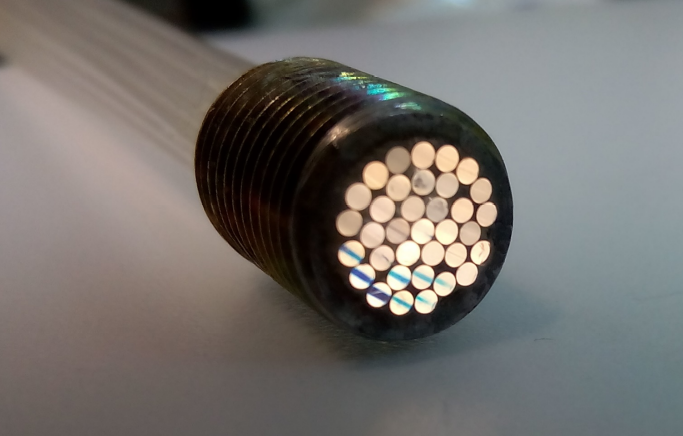
\includegraphics[width=\textwidth]{5Prototypes/52PreliminarPrototypes/521TritiumIFIC0/Metalic_piece_of_fiber_bundle.png}  
    \caption{Metalic piece of the fiber bundle. \label{subfig:MetalicPieceFiberBunchTritiumIFIC0}}
    \end{subfigure}
    \hfill
    \begin{subfigure}[b]{0.4\textwidth}
    \centering
    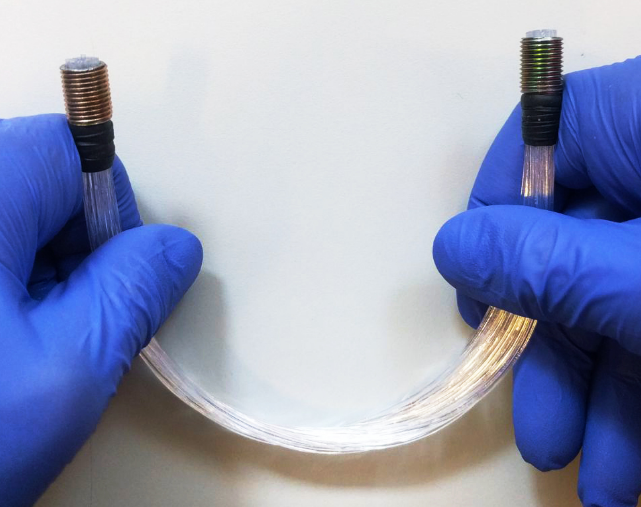
\includegraphics[width=\textwidth]{5Prototypes/52PreliminarPrototypes/521TritiumIFIC0/FiberBundleBent.png}  
    \caption{Fiber bundle in a position similar to the prototype.\label{subfig:FiberBunchTritiumIFIC0Bent}}
    \end{subfigure}
    \hfill
    \begin{subfigure}[b]{0.7\textwidth}
    \centering
    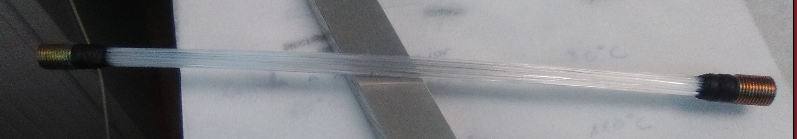
\includegraphics[width=\textwidth]{5Prototypes/52PreliminarPrototypes/521TritiumIFIC0/FiberBundleStraight.png}  
    \caption{Bundle of fibers in a straight position.\label{subfig:FiberBunchTritiumIFIC0}}
    \end{subfigure}
 \caption{Bundle of $35$ fibers, the length of which is $20~\cm$, used in TRITIUM-IFIC 0 prototype.}
 \label{fig:FiberBundleOfTritiumIFIC0}
\end{figure}

The fiber bundle was placed inside of a vessel, made of PVC\footnote{Polyvinyl Chloride, PVC}  since it is a safe material widely used. This vessel, shown in Figure \ref{fig:TritiumIFIC0}, was designed in a U-shape to improve the radiological safety, although this shape was not efficient for tritium detection as we learned afterwards. As can be seen in Figure \ref{fig:TritiumIFIC0}, a frame of methacrylate and steel was designed and built to hold the prototype. Two calibrated PMTs were optically coupled to the fiber bundle ends using optical grease \cite{OpticalGrease}. The employed PMTs were the model R8520-460 from Hamamatsu company \cite{DataSheetPMTs} and the high voltage between the dynodes was distributed by the electronic circuit show in fig  \ref{fig:VoltageDividerCircuit}. The high voltage was $-800~\volt$, at which their gain are $1.26 \cdot{} 10^6$ and $1.01 \cdot{} 10^6$ and their quantum efficiency are $29.76\%$ and $28.66\%$ respectively. Their signals were processed and analyzed by the electronics shown in Figure \ref{subfig:ElectronicConfiguraiton2PMT}.

\begin{figure}[h]
\centering
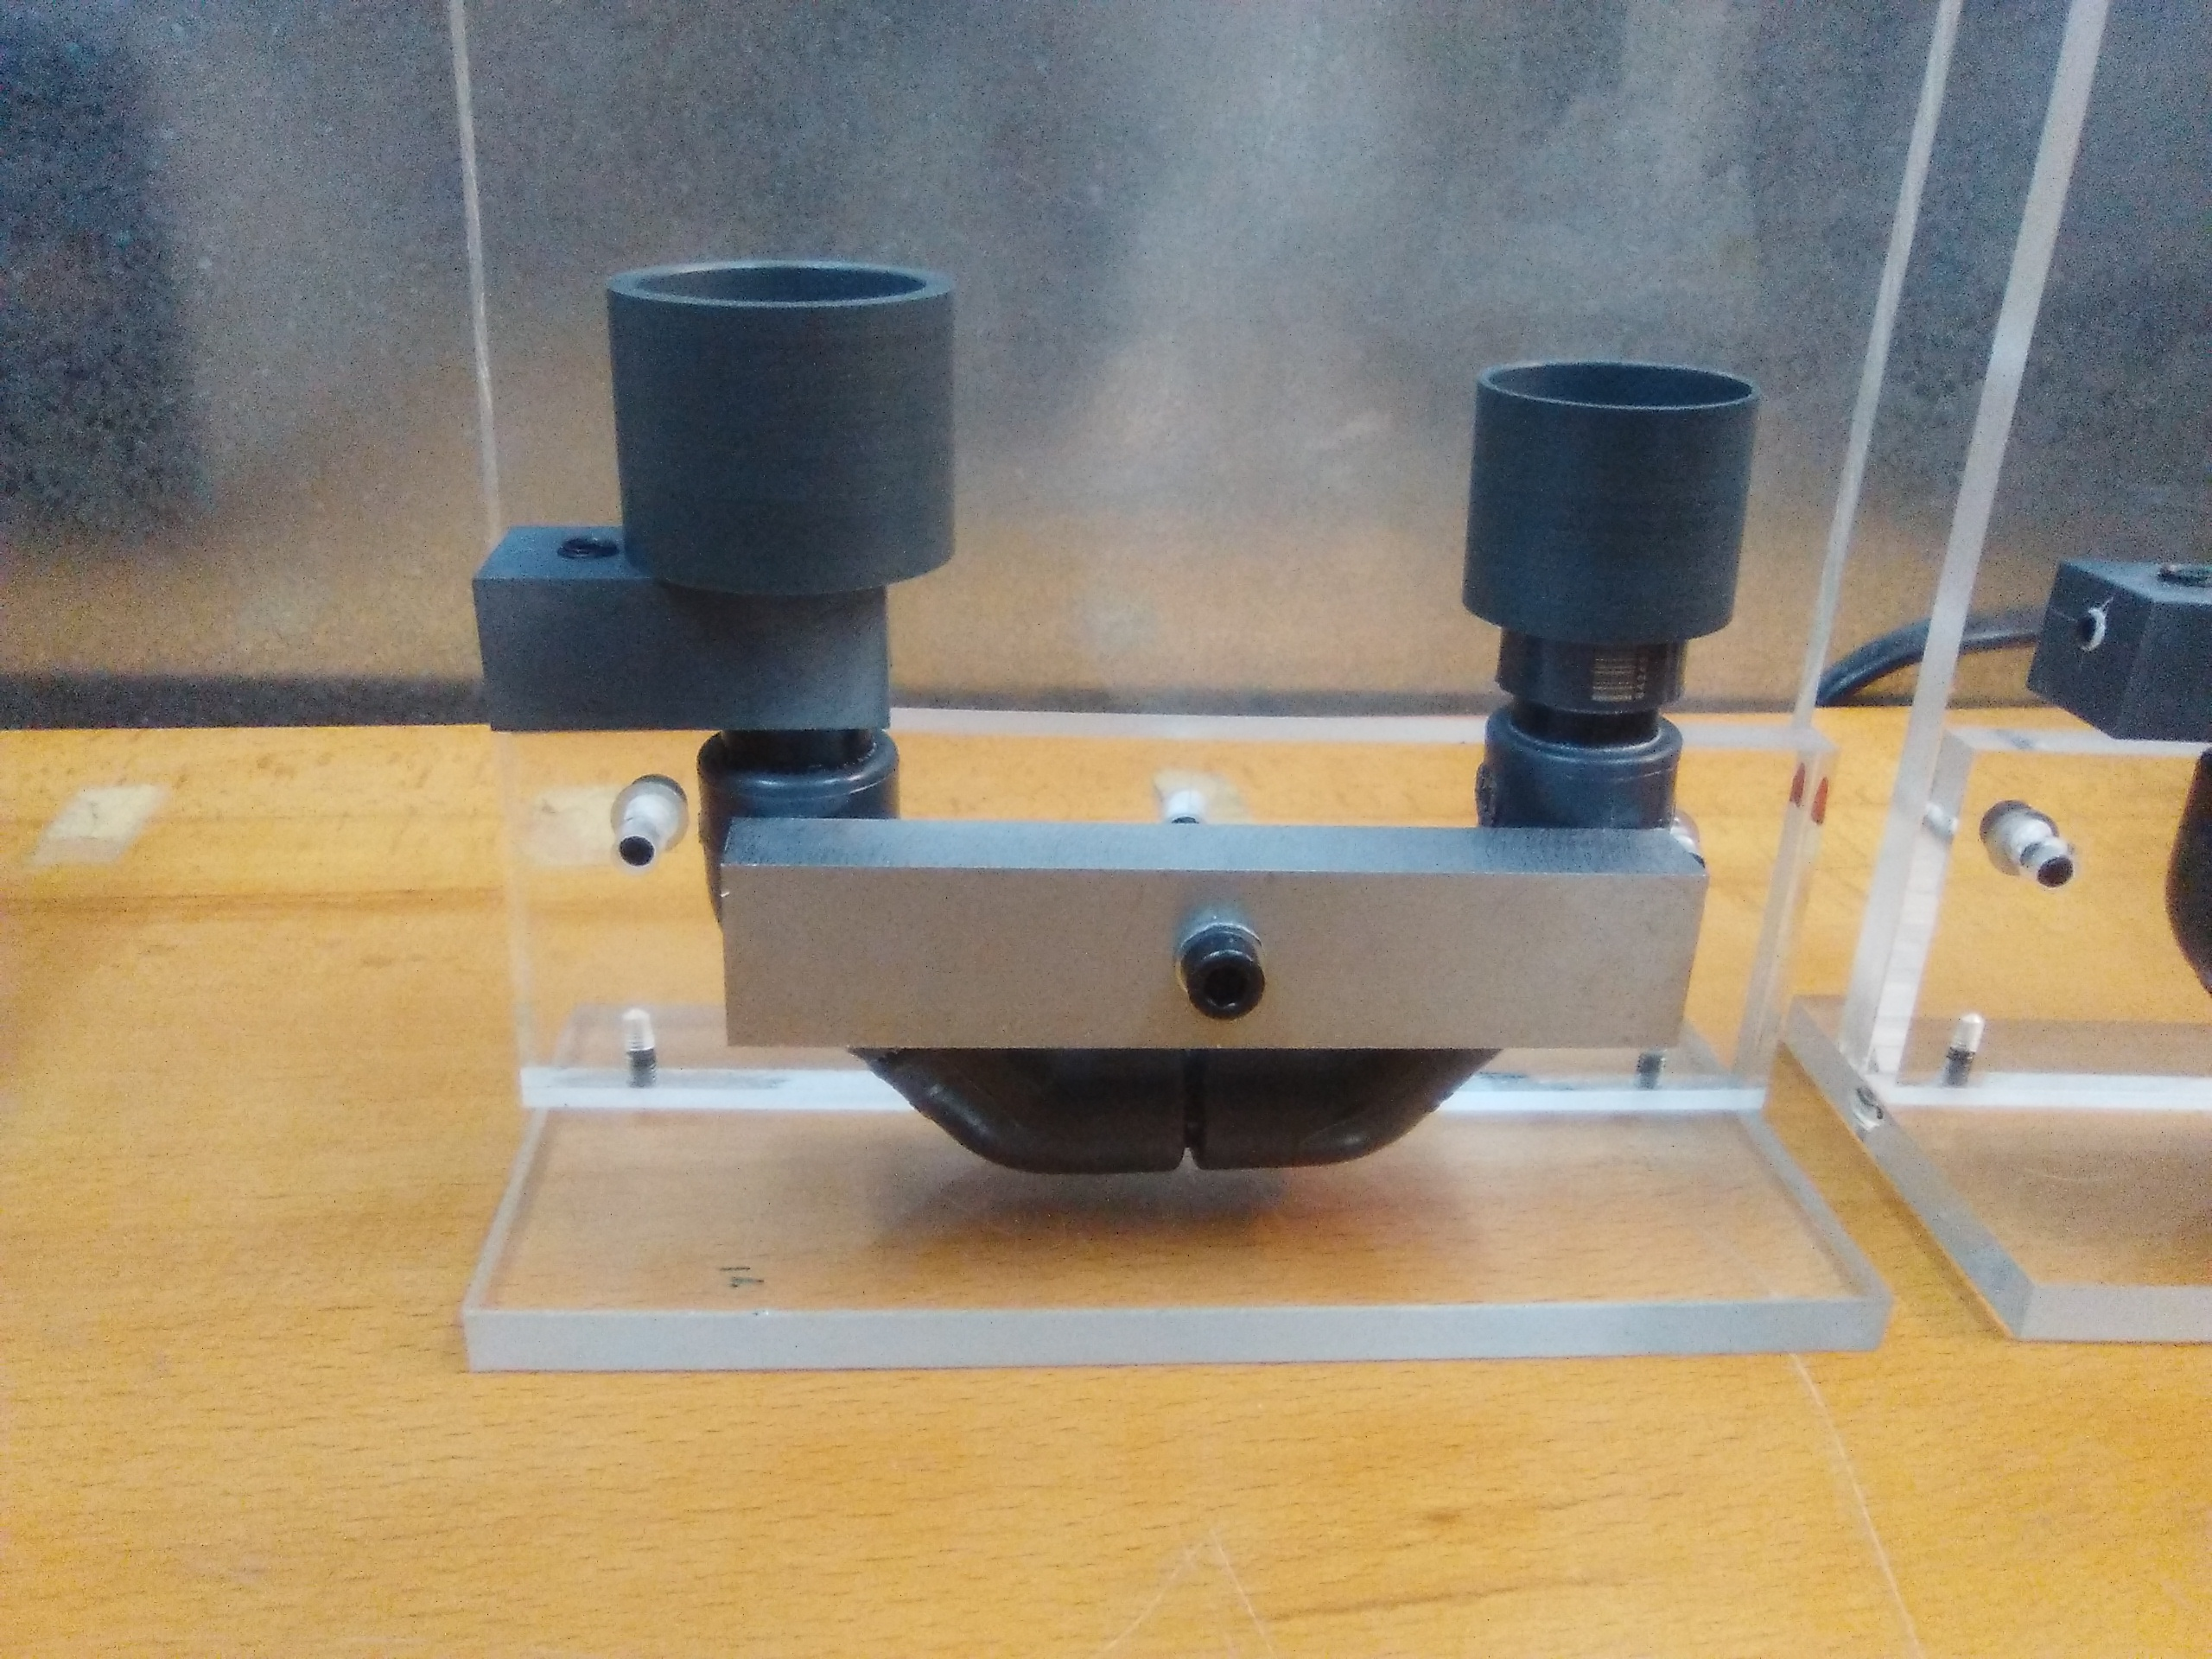
\includegraphics[scale=0.12]{5Prototypes/52PreliminarPrototypes/521TritiumIFIC0/Tritium_IFIC_0.jpg}
\caption{TRITIUM-IFIC 0 Prototype.\label{fig:TritiumIFIC0}}
\end{figure}

Two identical prototypes were built and filled following the same protocol. The first prototype, called TRITIUM-IFIC 0 Background, was filled with  ultrapure water ($39~\milli\liter$, uncertainty of $0.05\%$) and it was used to measure the radioactive background of the detector whereas the second prototype, called TRITIUM-IFIC 0 Signal, was filled with a radioactive liquid source of tritium, the preparation of which is reported in the appendix \ref{App:TritiumSourcePreparation}. The specific activity of the liquid source employed was $99.696~\kilo\becquerel/\liter$ (uncertainty of $2.24\%$) and the volume used to fill this prototype was the same, $39~\milli\liter$ (uncertainty of $0.05\%$). Therefore, the total activity of this tritiated water sample was approximately $3.888 \pm 0.087~\kilo\becquerel$. This second prototype was used to measure the signal of the detector (tritium + background), The measured tritium activity was determined by substracting the background from the signal. 

A statistically significant number of time coincident events was not found, so the measurement of time coincidences was not possible. The loss of photons could be caused for several reasons, such as an excessive curvature of the fiber bundle due to the U-shape of the PVC vessel, causing most of the photons escape from the fibers, or the poor quality of the tritiated water-fiber interface (the cleaning process described in section \ref{subsec:CleaningProcess} was motivated by this result). To avoid this problem and to obtain some data with this prototype, a measurement was performed with a single PMT. For this task, the electronic configuration shown in Figure \ref{subfig:ElectronicConfiguraiton1PMT} was used. The results of these measurements are reported in section \ref{subsec:ResultsTritiumIFIC0}.

An additional test was carried out to find an explanation of the absence of time coincident events in the data. A transparent glass vessel was built similar to the TRITIUM-IFIC 0 prototype vessel, shown in Figure \ref{subfig:PMMAVesselToTestLostPhotons}, to study the effect of the fiber bundle curvature. The LED described in section \ref{subsubsec:CharacterizationFibers} was used to verify the reduction in photocollection efficiency of the fiber bundle due to this curvature. As can be seen in Figure \ref{subfig:TestLostPhotons}, a large percentage of the photons are lost due to the curvature. This problem lead us to use a straight fiber arrangement in next prototypes.

\begin{figure}
\centering
    \begin{subfigure}[b]{0.45\textwidth}
    \centering
    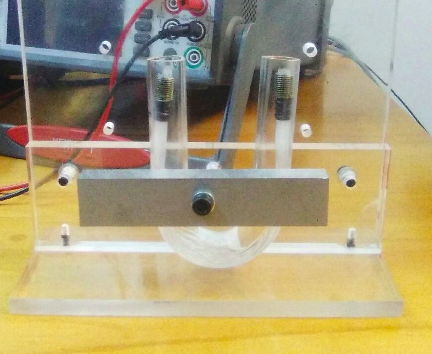
\includegraphics[width=\textwidth]{5Prototypes/52PreliminarPrototypes/521TritiumIFIC0/PMMA_vessel_ZOOM.png}  
    \caption{PMMA vessel.\label{subfig:PMMAVesselToTestLostPhotons}}
    \end{subfigure}
    \hfill
    \begin{subfigure}[b]{0.45\textwidth}
    \centering
    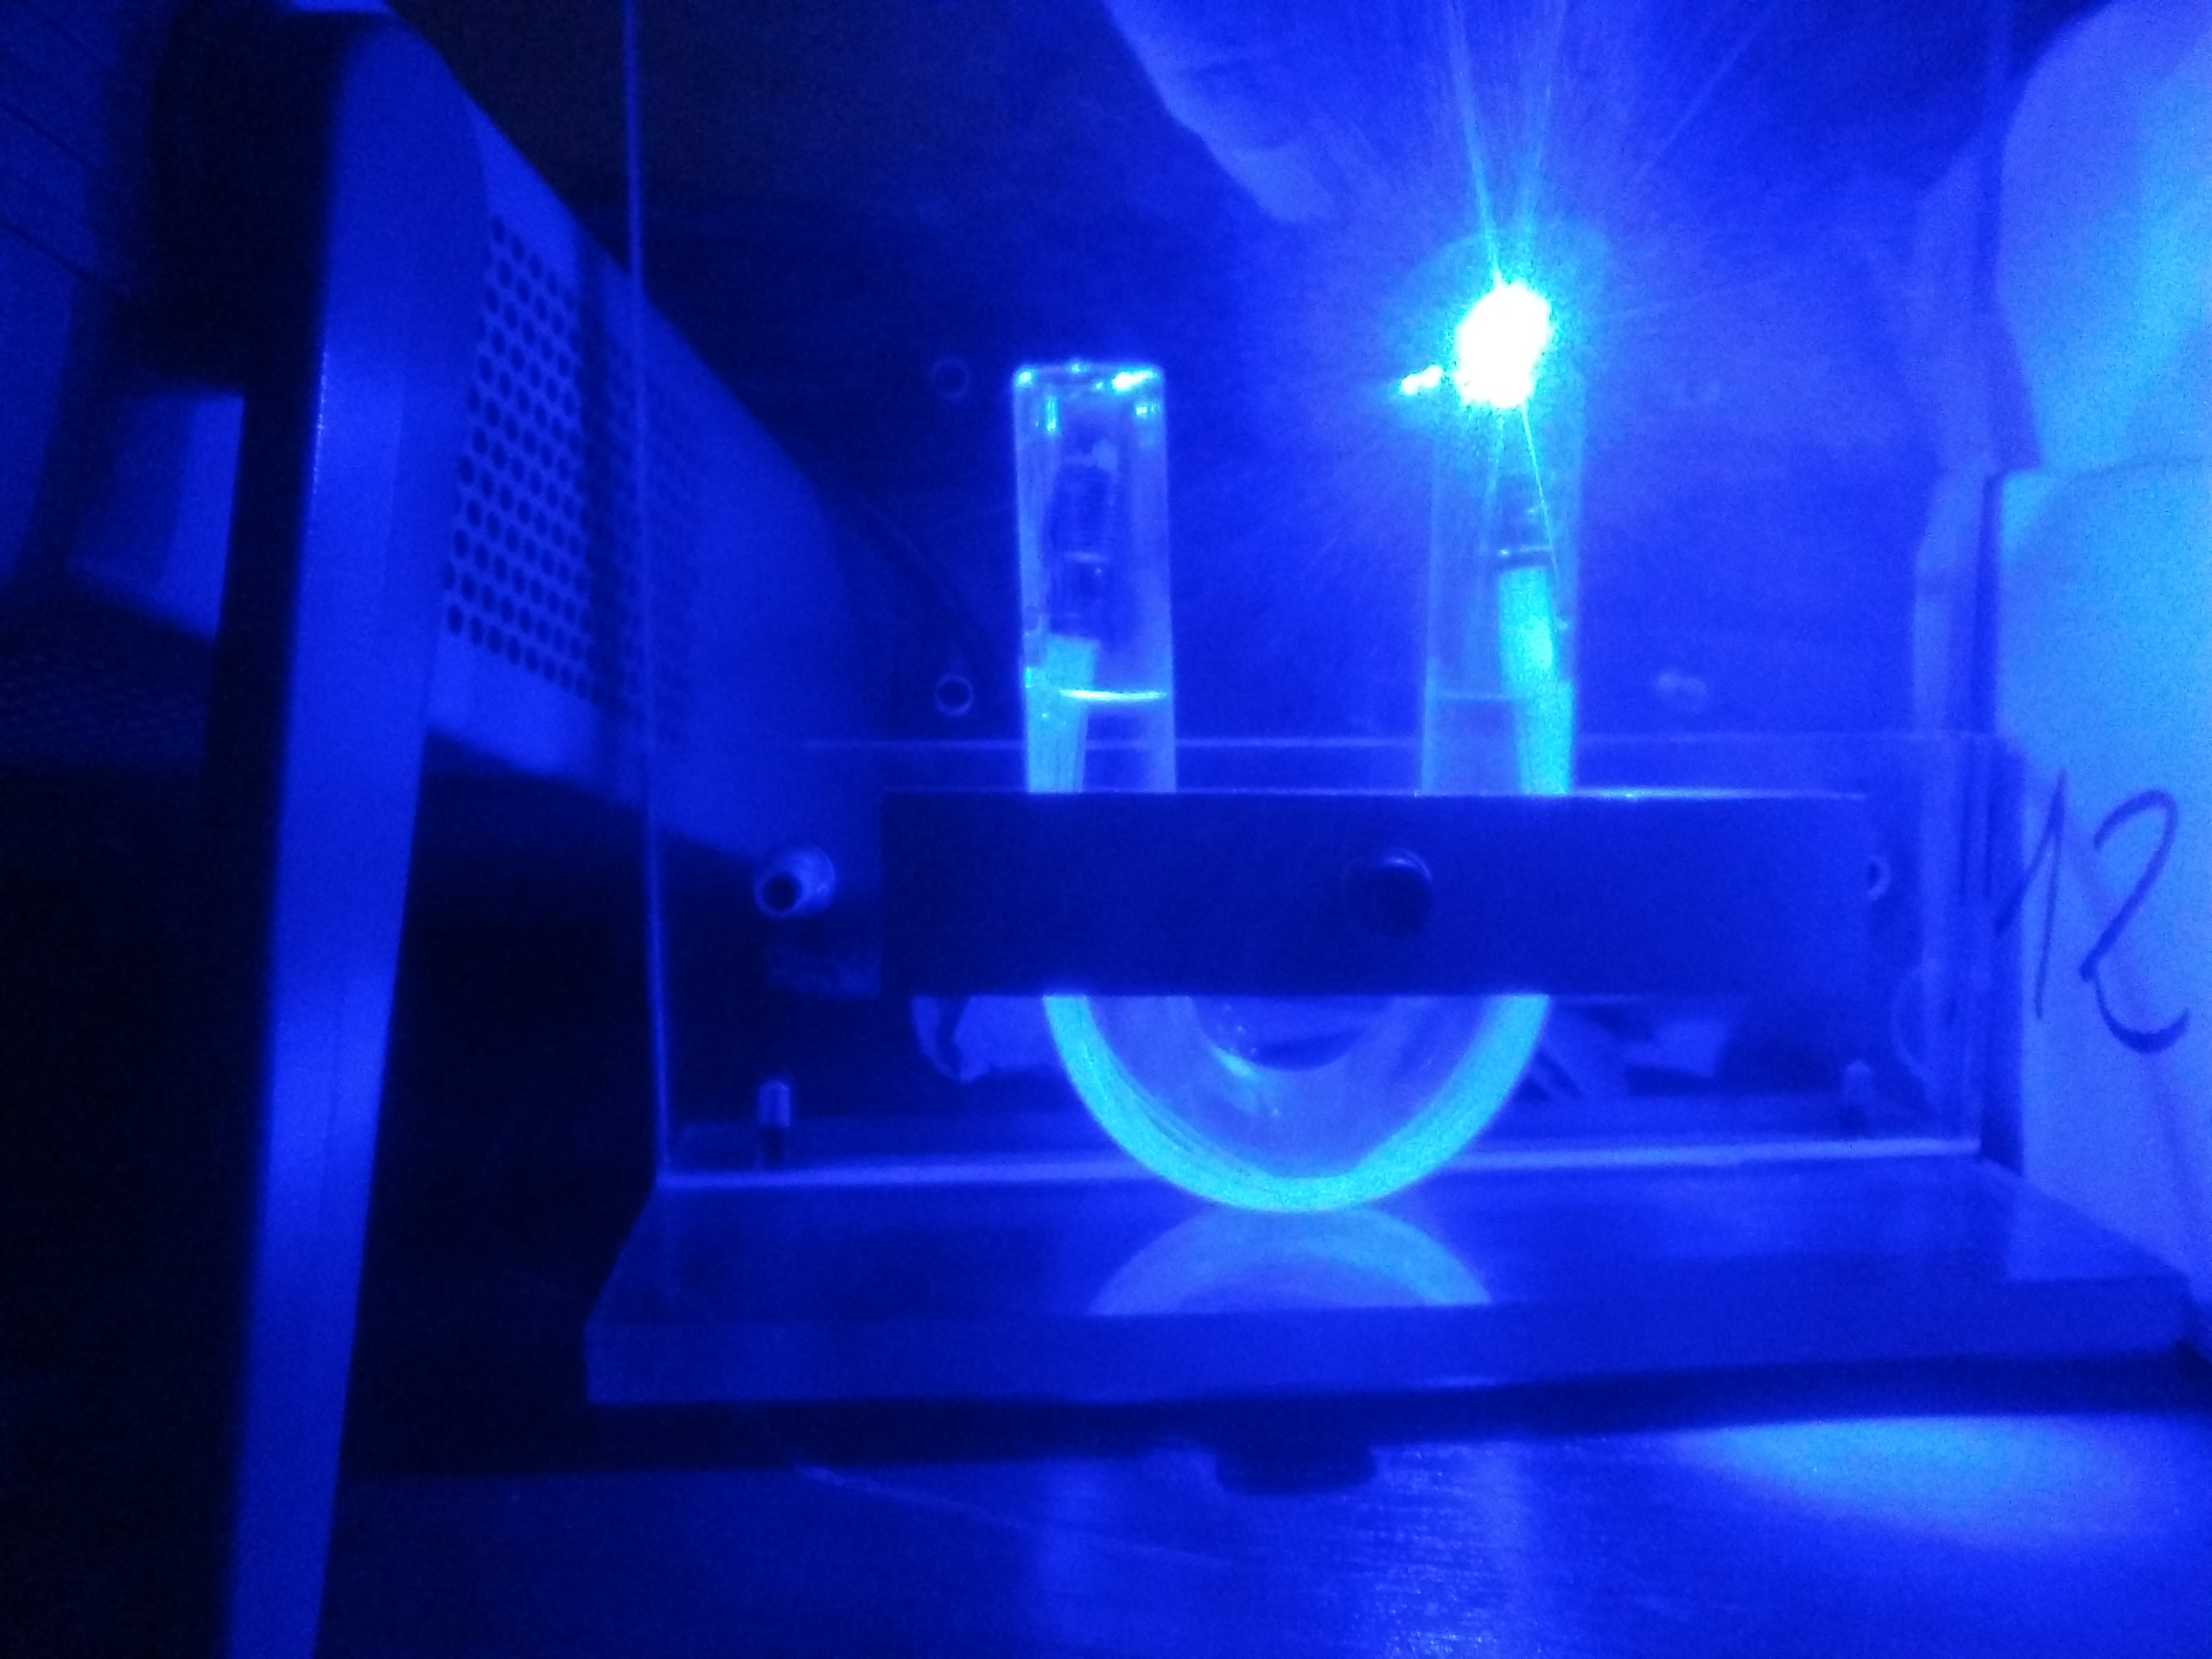
\includegraphics[width=\textwidth]{5Prototypes/52PreliminarPrototypes/521TritiumIFIC0/Lost_Photons.jpg}  
    \caption{Test performed to check the lost photons.\label{subfig:TestLostPhotons}}
    \end{subfigure}
 \caption{PMMA vessel used to check photon loss due to fiber bundle curve.}
 \label{fig:TestLostPhotons}
\end{figure}



%In addition, some improvements was applied to next prototype, Tritium-IFIC 1. On the one hand, the special cleaning protocol, previously explained in section \ref{subsubsec:CleaningProcess}, was applied on the fibers. It was used to improve the interfaces between fiber and tritiated water, creating a better wetting property of the fiber, which will result in more tritium events detected and a greater photon collection efficiency.

%On the other hand, as we have seen in our previous characterization study of the fibers, shown in section \ref{subsubsec:CharacterizationFibers}, the photon collection efficiency of the fibers used is poor, so a large number of photons will be lost in each tritium event.

%It is an innerent characteristic of the fiber which we cannot change but, to reduce its effect, we will use a Teflon vessel for our next prototypes.

%Teflon is an interesting material for its optical properties, specifically its reflection factor, which is very close to $100\%$ at the working wavelength. It means that practically all the photons that reach the walls of the vessel will be reflected back to the fiber.

%On the other hand, the fibers were inspected under the electronic microscope of the SCSIE \cite{ElectronicMicroscopeSCSIE}, with which we can see details of the order of tens of nanometers.

%The result is shown in Figure \ref{}, where you can see many irregularities of the order of $X~\nm$. These irregularities will cause photons to escape from the fiber. It is a characteristic of the fibers that we cannot change but, to reduce its effect, we will use a Teflon vessel for our next prototypes.

%FOTOOOO

%Teflon is an interesting material for its optical properties, specifically its reflection factor. Its reflection factor is very close to $100\%$ at the working wavelength, which means that practically all the photons that reach walls of the vessel will be reflected back to the fiber.